\documentclass{standalone}
\usepackage{tikz}
\usetikzlibrary{arrows.meta}
\begin{document}
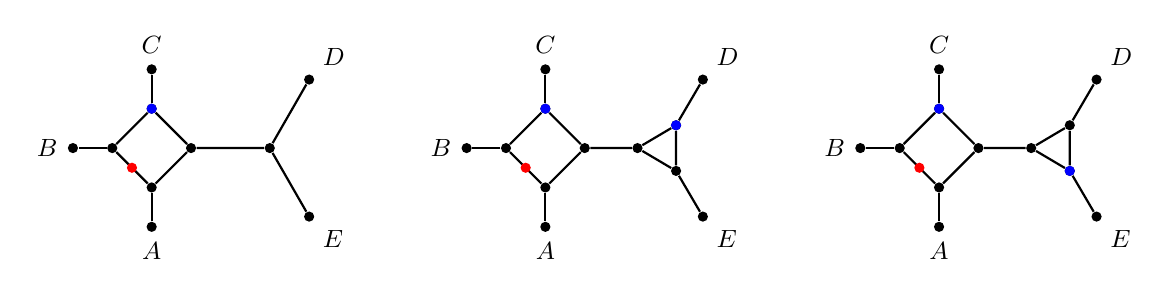
\begin{tikzpicture}[>=Stealth, every node/.style={font=\small},dot/.style={circle,fill=black,inner sep=1.3pt},leaf/.style={dot},int/.style={dot},]
\begin{scope}[shift={(0,0)}]
\node[int] (u0) at (0,-0.5) {};
\node[int] (u1) at (-0.5,0) {};
\node[int] (u2) at (0,0.5) {};
\node[int] (u3) at (0.5,0) {};
\node[int] (u4) at (1.5,0) {};
\node[leaf, label=below:$A$] (A) at (0,-1) {};
\node[leaf, label=left:$B$] (B) at (-1, 0) {};
\node[leaf, label=above:$C$] (C) at (0,1) {};
\node[leaf, label=above right:$D$] (D) at (2,0.87) {};
\node[leaf, label=below right:$E$] (E) at (2,-0.87) {};
\draw[line width=0.8pt] (u3) -- (u0) -- (u1) -- (u2) -- (u3) -- (u4);
\draw[line width=0.8pt] (u0) -- (A);
\draw[line width=0.8pt] (u1) -- (B);
\draw[line width=0.8pt] (u2) -- (C);
\draw[line width=0.8pt] (u4) -- (D);
\draw[line width=0.8pt] (u4) -- (E);
\node[circle,fill=red,inner sep=1.3pt] (root) at (-.25,-.25) {};
\node[circle,fill=blue,inner sep=1.3pt] at (0,.5) {};
\end{scope}
\begin{scope}[shift={(5,0)}]
\node[int] (u0) at (0,-0.5) {};
\node[int] (u1) at (-0.5,0) {};
\node[int] (u2) at (0,0.5) {};
\node[int] (u3) at (0.5,0) {};
\node[int] (u4) at (1.17,0) {};
\node[int] (u5) at (1.66,0.29) {};
\node[int] (u6) at (1.66,-0.29) {};
\node[leaf, label=below:$A$] (A) at (0,-1) {};
\node[leaf, label=left:$B$] (B) at (-1, 0) {};
\node[leaf, label=above:$C$] (C) at (0,1) {};
\node[leaf, label=above right:$D$] (D) at (2,0.87) {};
\node[leaf, label=below right:$E$] (E) at (2,-0.87) {};
\draw[line width=0.8pt] (u3) -- (u0) -- (u1) -- (u2) -- (u3) -- (u4) -- (u5) -- (u6) -- (u4);
\draw[line width=0.8pt] (u0) -- (A);
\draw[line width=0.8pt] (u1) -- (B);
\draw[line width=0.8pt] (u2) -- (C);
\draw[line width=0.8pt] (u5) -- (D);
\draw[line width=0.8pt] (u6) -- (E);
\node[circle,fill=red,inner sep=1.3pt] (root) at (-.25,-.25) {};
\node[circle,fill=blue,inner sep=1.3pt] at (0,.5) {};
\node[circle,fill=blue,inner sep=1.3pt] at (1.66,.29) {};
\end{scope}
\begin{scope}[shift={(10,0)}]
\node[int] (u0) at (0,-0.5) {};
\node[int] (u1) at (-0.5,0) {};
\node[int] (u2) at (0,0.5) {};
\node[int] (u3) at (0.5,0) {};
\node[int] (u4) at (1.17,0) {};
\node[int] (u5) at (1.66,0.29) {};
\node[int] (u6) at (1.66,-0.29) {};
\node[leaf, label=below:$A$] (A) at (0,-1) {};
\node[leaf, label=left:$B$] (B) at (-1, 0) {};
\node[leaf, label=above:$C$] (C) at (0,1) {};
\node[leaf, label=above right:$D$] (D) at (2,0.87) {};
\node[leaf, label=below right:$E$] (E) at (2,-0.87) {};
\draw[line width=0.8pt] (u3) -- (u0) -- (u1) -- (u2) -- (u3) -- (u4) -- (u5) -- (u6) -- (u4);
\draw[line width=0.8pt] (u0) -- (A);
\draw[line width=0.8pt] (u1) -- (B);
\draw[line width=0.8pt] (u2) -- (C);
\draw[line width=0.8pt] (u5) -- (D);
\draw[line width=0.8pt] (u6) -- (E);
\node[circle,fill=red,inner sep=1.3pt] (root) at (-.25,-.25) {};
\node[circle,fill=blue,inner sep=1.3pt] at (0,.5) {};
\node[circle,fill=blue,inner sep=1.3pt] at (1.66,-.29) {};
\end{scope}
\end{tikzpicture}
\end{document}